\SACCMD{taper}
\label{cmd:taper}

\SACTitle{概要}
在数据两端应用对称的taper函数,使得数据在两端平滑地衰减到零

\SACTitle{语法}
TAPER [ TYPE HANNING | HAMMING | COSINE ] [ WIDTH v ]

\SACTitle{输入}
\begin{itemize}
\item TYPE HANNING|HAMMIN|COSINE : 应用Hanning、Hamming、余弦衰减窗
\item WIDTH v : 设置位于数据首末两端的衰减窗的宽度为v,这个值在0.0和0.5之间
\end{itemize}

\SACTitle{缺省值}
TAPER TYPE HANNING WIDTH 0.05

\SACTitle{说明}
taper函数是在0和1之间取值的单调变化的函数。它对称地施加于数据的首尾两端。
对于数据的首端,taper函数的第一个点\footnote{究竟是第0个点还是第1个点,这个
问题比较纠结,当初从FORTRAN改写成SAC的时候,遗留下来一些历史问题。}值为0,第NPTS*WIDTH个点的值为1
(NPTS为数据总点数,WIDTH为命令中设置的参数\footnote{这下知道为什么WIDTH只能取0.0-0.5了吧。})。
将taper函数与数据相乘即使得数据的首端从0开始不断光滑地增加到其原始值。数据
末端完全类似,只是数据由其原始值不断光滑地减小到0。正如taper的英译,``逐渐
消失'',有时候也翻译为``尖灭''。

taper命令的本质如下式所示:
\begin{displaymath}
Data(j) = \left\{
		  \begin{array}{ll}
		  Data(j)*Taper(j) & \textrm{j $\in$ [1,\ npts*width]} \\
		  Data(j)*Taper(npts-j) & \textrm{j $\in$ [npts-npts*width,\ npts]} \\
		  \end{array}
\right.
\end{displaymath}

其中taper函数可以表示为:
\[ Taper(j)=F_0 - F_1\cos(\omega(j-1))	\quad j \in [1,\ npts*width] \]

下表定义了不同的衰减的各种参数。在这个表中,N为首尾两端的衰减数据的长度,即NPTS*WIDTH。

\begin{center}
\begin{tabular}{llll}
\toprule
类型 & $\omega$ & $F_0$	& $F_1$	\\
\midrule
HANNING	&	$\frac{\pi}{N}$	&	0.50	&	0.50	\\
HAMMING	&	$\frac{\pi}{N}$	&	0.54	&	0.46	\\
COSINE	&	$\frac{\pi}{2N}$	&	1.00	&	1.00	\\
\bottomrule
\end{tabular}
\end{center}

\begin{figure}[h]
\caption{Taper函数对比图}
\centering
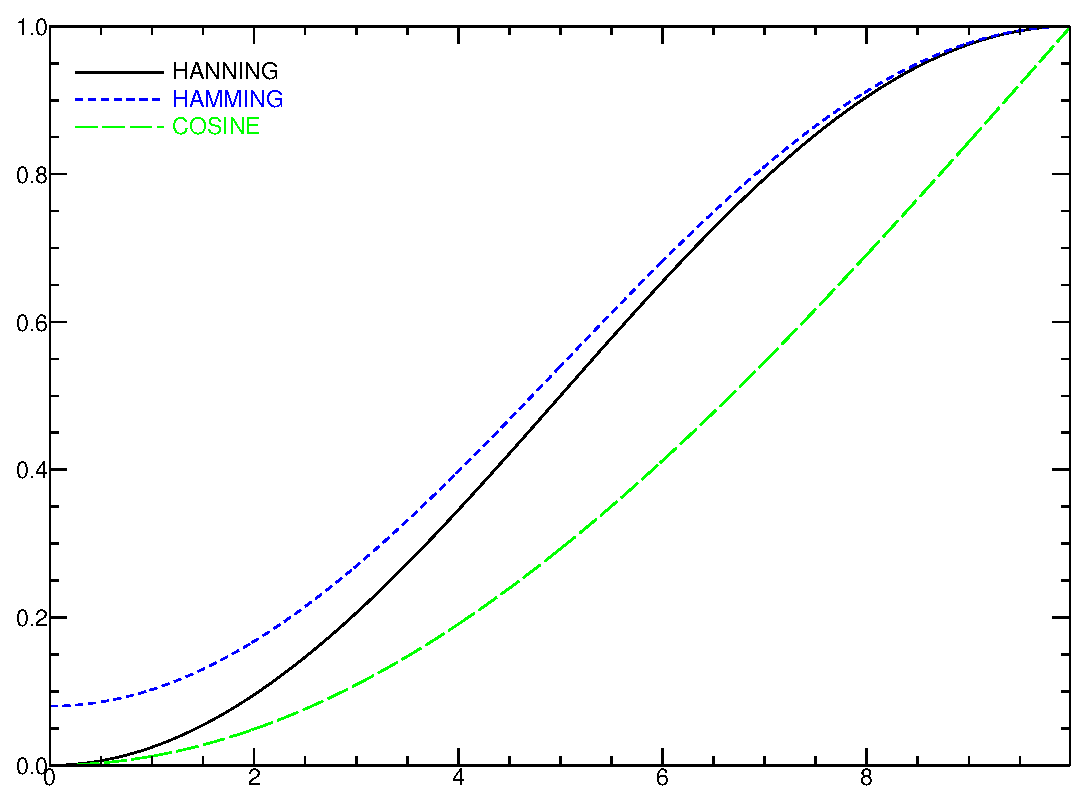
\includegraphics[width=8cm]{taper}
\end{figure}

\SACTitle{错误消息}
\begin{itemize}
\item[-]1301: 未读入数据文件
\item[-]1306: 对不等间隔文件的非法操作
\end{itemize}

\SACTitle{头段变量改变}
DEPMIN, DEPMAX, DEPMEN

\SACTitle{最近修订}
January 15, 1985 (Version 9.10)
